%-------------------------------------------------------------------------------------------------
\section{Conclus�es} 
%-------------------------------------------------------------------------------------------------

\begin{frame}
\frametitle{Conclus�es}

\begin{itemize}
	\item Utiliza��o de algoritmos de identifica��o de sistemas n�o lineares pode ser estendida para a identifica��o de
	controladores n�o lineares.
	\item Refer�ncia virtual traz diversas vantagens para a obten��o dos dados para alimenta��o dos algoritmos n�o
	lineares.
	\item Resultados obtidos com os exemplos apresentados podem ser considerados satisfat�rios para um grande n�mero de
	aplica��es.
\end{itemize}
\end{frame}

%-------------------------------------------------------------------------------------------------
%-------------------------------------------------------------------------------------------------

\begin{frame}
	\frametitle{Quest�es}
			\linespread{1.3}
\centerline{Muito Obrigado}
\end{frame}

%-------------------------------------------------------------------------------------------------
%-------------------------------------------------------------------------------------------------
% Slides extras
%-------------------------------------------------------------------------------------------------
%\subsection{Sinais utilizados} 
%-------------------------------------------------------------------------------------------------
\begin{frame}
\frametitle{Defini��es}
\framesubtitle{Sinal PRBS}
 
\begin{block}{Sinal PRBS}
\begin{equation}
u(t)=rem(A(z)u(t), 2)=rem(a_1 u(t-1)+...+a_n u(t-n), 2)
\nonumber
\end{equation}
\end{block}

\begin{columns}
\column{0.35\textwidth}

\begin{table}
\fontsize{6}{8}\selectfont
\begin{center}
\begin{tabular}{ccc}
\hline
        Ordem $n$ & $M=2^n-1$ & $a_k$ n�o   \\
        & & zeros para $k$ \\
\hline
        2       & 3        & 1, 2       \\
        3       & 7        & 2, 3       \\
        4       & 15       & 1, 4       \\
        5       & 31       & 2, 5       \\
        6       & 63       & 1, 6       \\
        7       & 127      & 3, 7       \\
        8       & 255      & 1, 2, 7, 8 \\
        9       & 511      & 4, 9       \\
        10      & 1023     & 7, 10      \\
        11      & 2047     & 9, 11      \\
\hline
\end{tabular}
\end{center}
\end{table}

\column{0.7\textwidth}
\begin{figure}[htbp]
	\center
	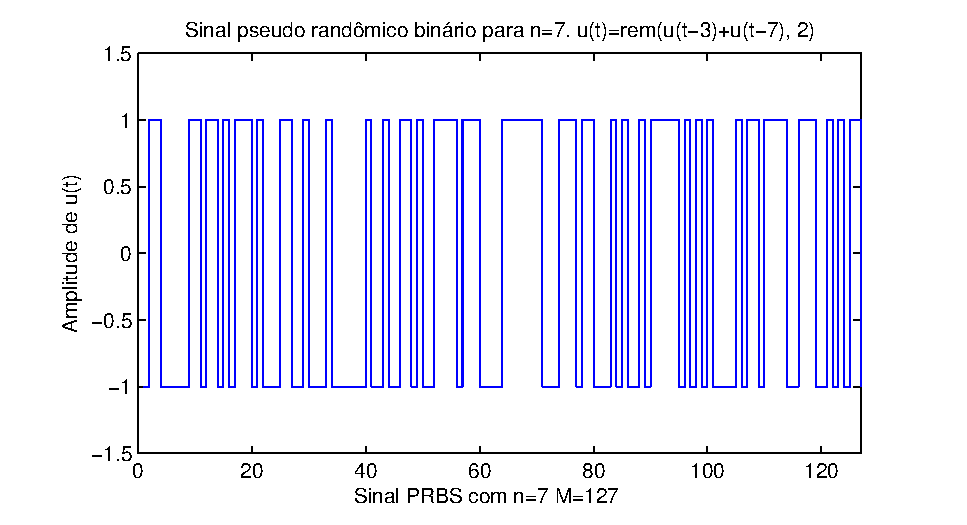
\includegraphics[width=0.95\columnwidth]{figures/si_project_prbs.eps}
	\caption{Sinal PRBS para $n=7$}
	\label{fig:si_project_prbs}
\end{figure}
\end{columns}
\end{frame}

